\documentclass[italian,12pt]{article}

\def\Title{Verbale interno}
\def\Subtitle{Riunione interna settimanale}
\def\Author{7Last}
\def\Date{2024-05-22}
\def\Version{v1.0}

%pacchetti extra da scaricare dblfloatfix, fancyhdr
\usepackage[left=2cm, right=2cm, bottom=3cm, top=3cm]{geometry}
\usepackage{fancyhdr}%creazione header-footer
\usepackage{graphicx} %serve per inserire immagini
\graphicspath{ {../../../logo/} }
%\usepackage{dblfloatfix} %serve per posizionare gli elementi dove si vuole
\usepackage[hidelinks]{hyperref} %serve per i link
\usepackage{tikz}
\usepackage{tgadventor} % font
\usepackage[useregional=numeric,showseconds=true,showzone=false]{datetime2}
\usepackage{caption}

\usepackage{hyperref}
\usepackage{tocloft}
\usepackage{titlesec}
\usepackage{color}
\usepackage{ulem}
\usepackage{pgfplots}
\usepackage{pgf-pie}
\usepackage[italian]{babel}
\usepackage{comment}
\usepackage{tabularx}
\usepackage{longtable}
\usepackage{float}
\usepackage{amsmath}

\linespread{1.2}
\captionsetup[table]{name=Tabella}
\geometry{headsep=1.5cm}

\renewcommand{\contentsname}{Indice}
\renewcommand\familydefault{\sfdefault}
\renewcommand{\listtablename}{Indice delle tabelle}
\renewcommand\familydefault{\sfdefault}
\renewcommand{\listfigurename}{Indice delle immagini}
\renewcommand\familydefault{\sfdefault}

% set sfdefault for page numbers
\let\oldthepage\thepage
\renewcommand{\thepage}{\sffamily\oldthepage}

\begin{document}
\newgeometry{left=2cm,right=2cm,bottom=2.1cm,top=2.1cm}
\begin{titlepage}
    \vspace*{.5cm}

    \vspace{2cm}
    {
        \centering
        {\bfseries\huge \Title\par}
        \bigbreak
        {\bfseries\large \Author\par}
        \bigbreak
        {\Version\par}
        \vfill

        \begin{tikzpicture}[remember picture,overlay]

            \fill[blue!20!black] (current page.south west) -- ++(10cm,0) -- ++(-10cm,15cm) -- cycle;
            \fill[orange] (current page.south east) -- ++(-18cm,0) -- ++(21.6cm,22cm) -- cycle;

            \clip (0,-3cm) circle (2.5cm) node (current page.center) {
\includegraphics[width=5cm]{logo.jpg}};
        \end{tikzpicture}

    }

    \vfill

\end{titlepage}

\restoregeometry





















\newpage
%---------------header------------------%
\pagestyle{fancy}
\fancyhead{} % pulizia degli header
\lhead{%
\begin{tikzpicture}
    \clip (0,0) circle (0.5cm);
    \node at (0,0) {
\includegraphics[width=1cm]{logo}};
\end{tikzpicture}%
}
\chead{\vspace{\fill}\Title\vspace{\fill}}
\rhead{\vspace{\fill}\Version\vspace{\fill}}
%quad è una spaziatura
%---------------------------------------%

\begin{table}[!h]
	\caption*{Versioni}
	\begin{center}
		\begin{tabular}{ c c c c p{6.1cm} }
			\hline                                                                                                 \\[-2ex]
			Ver. & Data       & Redattore          & Verificatore      & Descrizione                                    \\
			\\[-2ex] \hline \\[-1.5ex]
			0.1  & 2024-05-08 & Valerio Occhinegro &                   & Prima Stesura \\
			\\[-1.5ex] \hline
		\end{tabular}
	\end{center}
\end{table}

\newpage
\tableofcontents
\listoftables
\listoffigures
\newpage

\section{Introduzione}
\subsection{Obiettivo del documento}
Il presente documento ha lo scopo di definire le strategie di verifica e validazione utilizzate per assicurare il corretto funzionamento dello strumento sviluppato e delle
attività che lo accompagnano.  Sarà sottoposto a revisioni continue, così da prevedere situazioni precedentemente non occorse e da seguire l'evoluzione del progetto.
\subsection{Glossario}
Il \href{https://7last.github.io/docs/rtb/documentazione-interna/glossario#glossario}{glossario\textsubscript{G}} è uno strumento utilizzato per risolvere eventuali dubbi riguardanti 
alcuni termini specifici utilizzati nella redazione del documento.
Esso conterrà la definizione dei termini evidenziati e sarà consultabile al seguente \href{https://7last.github.io/docs/rtb/documentazione-interna/glossario}{link}. I termini presenti in tale documento saranno evidenziati da una 'G' a pedice.
\subsection{Riferimenti}
\subsubsection{Riferimenti normativi}
\begin{itemize}
    \item \href{https://7last.github.io/docs/rtb/documentazione-interna/glossario#norme-di-progetto}{Norme di progetto\textsubscript{G}} (aggiungere versione e/o link al documento);
    \item Regolamento del progetto:\\
		  \url{https://www.math.unipd.it/~tullio/IS-1/2023/Dispense/PD2.pdf}.
\end{itemize}
\subsubsection{Riferimenti informativi}
\begin{itemize}
    \item \href{https://7last.github.io/docs/rtb/documentazione-interna/glossario#capitolato}{Capitolato\textsubscript{G}} d'appalto C6: \href{https://7last.github.io/docs/rtb/documentazione-interna/glossario#synccity}{SyncCity\textsubscript{G}} – A \href{https://7last.github.io/docs/rtb/documentazione-interna/glossario#smart-city}{smart city\textsubscript{G}} monitoring platform\\
    \url{https://www.math.unipd.it/~tullio/IS-1/2023/Progetto/C6.pdf};
    \item \href{https://it.wikipedia.org/wiki/ISO/IEC_9126}{Standard ISO/IEC 9126};
    \item \href{https://iso25000.com/index.php/en/iso-25000-standards/iso-25010}{Standard ISO/IEC 25010};
    \item \href{ https://en.wikipedia.org/wiki/ISO/IEC_12207}{Standard ISO/IEC 12207:1995};
    \item \href{URL}{\textit{Verbali esterni}};
    \item \href{URL}{\textit{Verbali interni}};
    \item \href{URL}{\href{https://7last.github.io/docs/rtb/documentazione-interna/glossario#analisi-dei-requisiti}{\textit{Analisi dei requisiti}\textsubscript{G}}};
    \item AGGIUNGERE LINK
\end{itemize}

\section{Requisiti dei workload OLAP}
In questa sezione viene riportato un elenco delle caratteristiche che compongono un database OLAP:
\begin{itemize}
	\item la vasta maggioranza delle richieste sono di lettura;
	\item i dati sono inseriti in batch di grandi dimensioni ($>1000$ righe);
	\item i dati sono aggiunti al DB e non modificati;
	\item le tabelle contengono un’alta quantità di colonne; 
	\item le query sono operazioni rare (solitamente centinaia per server);
	\item i valori contenuti nelle colonne sono relativamente piccoli: numeri e stringhe di piccole dimensioni;
	\item le transazioni non sono necessarie;
	\item bassi requisiti di consistenza dei dati;
	\item Il peso del risultato delle query è significativamente più contenuto rispetto a quello dei dati inseriti nel database. I dati sono filtrati o aggregati per essere aggiunti all’ interno della RAM di un singolo server.
\end{itemize}

















\section{Architettura di ClickHouse}
Gli elementi architettonici elencati nelle sottosezioni sono stati implementati dal team di \href{https://7last.github.io/docs/pb/documentazione-interna/glossario\#clickhouse}{ClickHouse\textsubscript{G}} per rispettare i requisiti OLAP. 
\subsection{Archiviazione compressa e orientata alle colonne}
\href{https://7last.github.io/docs/pb/documentazione-interna/glossario\#clickhouse}{ClickHouse\textsubscript{G}} sfrutta un sistema che consente di archiviare le colonne contenenti la stessa tipologia di dato nello stesso luogo. Questa soluzione rende possibile una migliore compressione e velocizza notevolmente le query.


\subsection{Table engines}
Le table engines determinano la tipologia di tabelle e le features che saranno disponibili per processare i dati contenuti al loro interno.
La più utilizzata è la mergetree table engine che rappresenta il metodo base di scrittura e combinazione dei dati. Quasi tutte le altre table engine derivano dalla MergeTree. 
MergeTree consente di scrivere e archiviare i dati su file immutabili chiamati “parts”. I file sono processati in background e uniti in un file più grande con l’obiettivo di ridurre la quantità di parts presenti su disco (meno file= letture più rapide).
Tutte le colonne contenute in una tabella sono salvate in parts differenti, e ogni dato è salvato seguendo l’ordine della chiave primaria; in questa maniera la lettura dei dati sarà più efficiente.


\subsection{Indici}
\href{https://7last.github.io/docs/pb/documentazione-interna/glossario\#clickhouse}{Clickhouse\textsubscript{G}} utilizza solo due tipi di indici: primari e secondari.
Visto che tutti i dati sono salvati in ordine di chiave primaria, l’indice primario archivia il valore della chiave primaria in ogni N-riga. Questo ha lo scopo di salvare l’indice nella memoria per ottenere un’alta velocità di processazione. 


\subsection{Vector computation engine}
Grazie ai vector algorithms \href{https://7last.github.io/docs/pb/documentazione-interna/glossario\#clickhouse}{ClickHouse\textsubscript{G}} può elaborare dati contenuti in decine di migliaia di righe per colonna. Inoltre, gli algoritmi consentono di scrivere codice più efficiente che sfrutta i processori SIMD (Single Instruction stream, Multiple Data stream:struttura che consiste in un elevato numero di processori identici che eseguono la stessa sequenza di istruzioni su insiemi di diversi di dati) e tiene codice e dati vicini per avere dei pattern di accesso alla memoria migliori.

















\section{Limitazioni di ClickHouse}
In questa sezione vengono elencate le limitazioni che ClickHouse ha rispetto a TimescaleDB: 
\begin{itemize}
	\item performance peggiori rispetto a TimescaleDB in quasi tutte le query testate ad eccezione delle query eseguite su aggregazioni complesse;
	\item insert poco efficienti e utilizzo molto più alto del disco (2.7 volte maggiore rispetto a TImescale) in caso di  piccoli batch (100-300 righe/batch);
	\item il linguaggio di query non rispetta lo standard SQL e ha delle limitazioni (ad esempio la disincentivazione nell’utilizzo di join)
	\item mancanza di alcune funzionalità presenti in altri database SQL: no transactions, no correlated sub-queries, no stored procedures, no user-defined functions, no index management beyond primary and secondary indexes, no triggers; 
	\item impossibilità di modifica o cancellazione di dati ad alto tasso e bassa latenza, è necessario creare dei batch di eliminazioni e aggiornamenti;
	\item gli update e le cancellazioni in batch avvengono in maniera asincrona, a causa di ciò è difficile assicurare backup consistenti (l’unica maniera per avere un backup consistente è arrestare la scrittura sul database);
	\item la mancanza di transazioni e consistenza dei dati affligge anche le materialized views poiché il server non può aggiornare atomicamente più tabelle alla volta;
\end{itemize}

















\section{\textit{Benchmark}}
Seguono i risultati dei \textit{benchmark} effettuati dal team di sviluppo di TimescaleDB, che confrontano
le prestazioni dei due strumenti.

\begin{center}
	\includegraphics[width=0.85\textwidth]{imgs/01-timescale-vs-\href{https://7last.github.io/docs/pb/documentazione-interna/glossario\#clickhouse}{clickhouse\textsubscript{G}}.png}
	\captionof{figure}{\href{https://www.timescale.com/blog/what-is-clickhouse-how-does-it-compare-to-postgresql-and-timescaledb-and-how-does-it-perform-for-time-series-data/}{\href{https://7last.github.io/docs/pb/documentazione-interna/glossario\#clickhouse}{ClickHouse\textsubscript{G}} ha performance migliori di TimescaleDB con batch di dimensione superiore a 5,000 righe}}
\end{center}

\begin{center}
	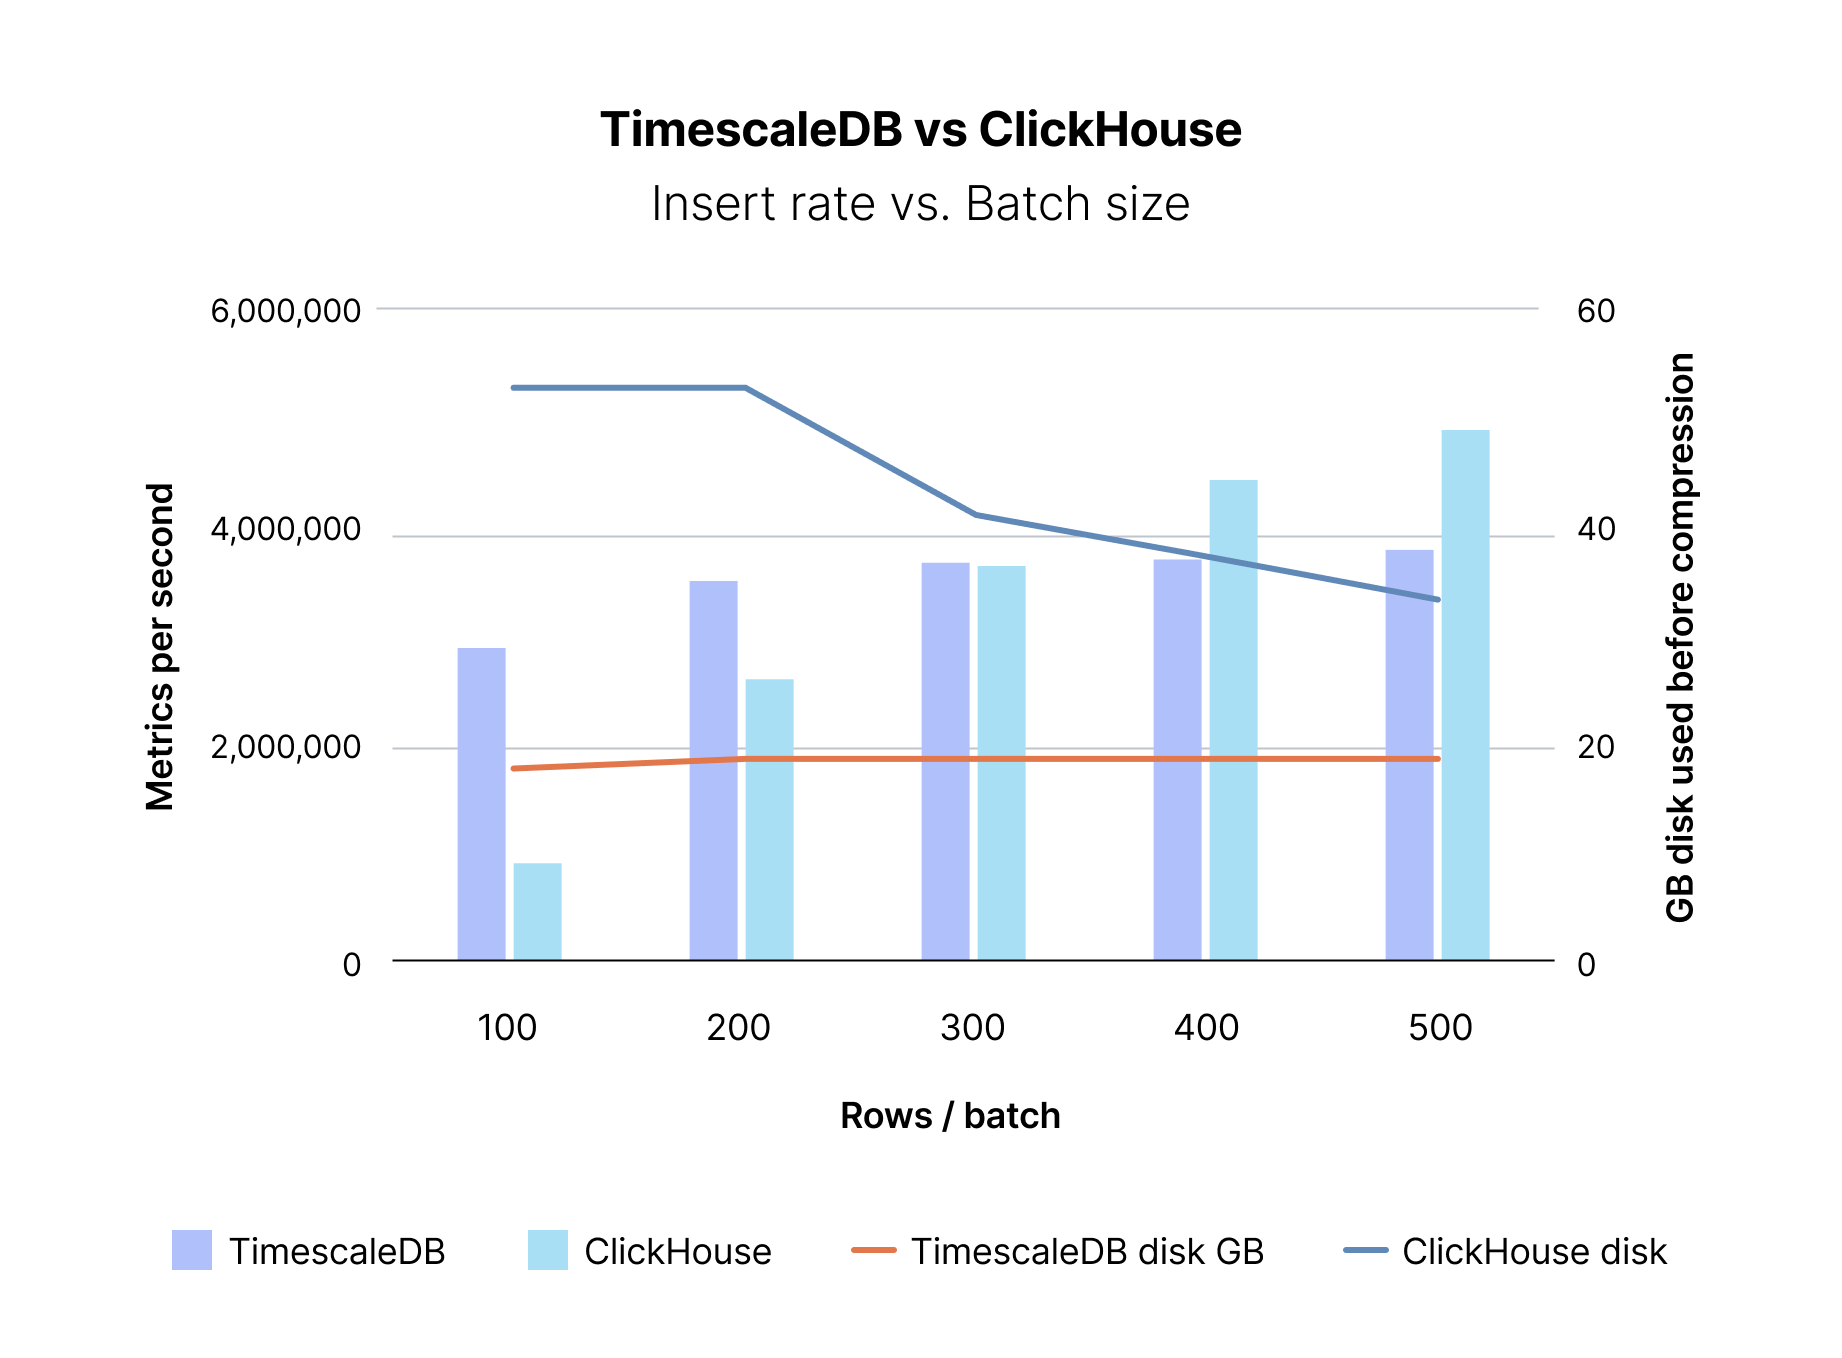
\includegraphics[width=0.85\textwidth]{imgs/02-small-batch-insert-performance.png}
	\captionof{figure}{\href{https://www.timescale.com/blog/what-is-clickhouse-how-does-it-compare-to-postgresql-and-timescaledb-and-how-does-it-perform-for-time-series-data/}{Timescale ha performance migliori di \href{https://7last.github.io/docs/pb/documentazione-interna/glossario\#clickhouse}{ClickHouse\textsubscript{G}} con batch di dimensione più contenuta e usa una quantità di disco inferiore di 2.7 volte}}
\end{center}

\begin{center}
	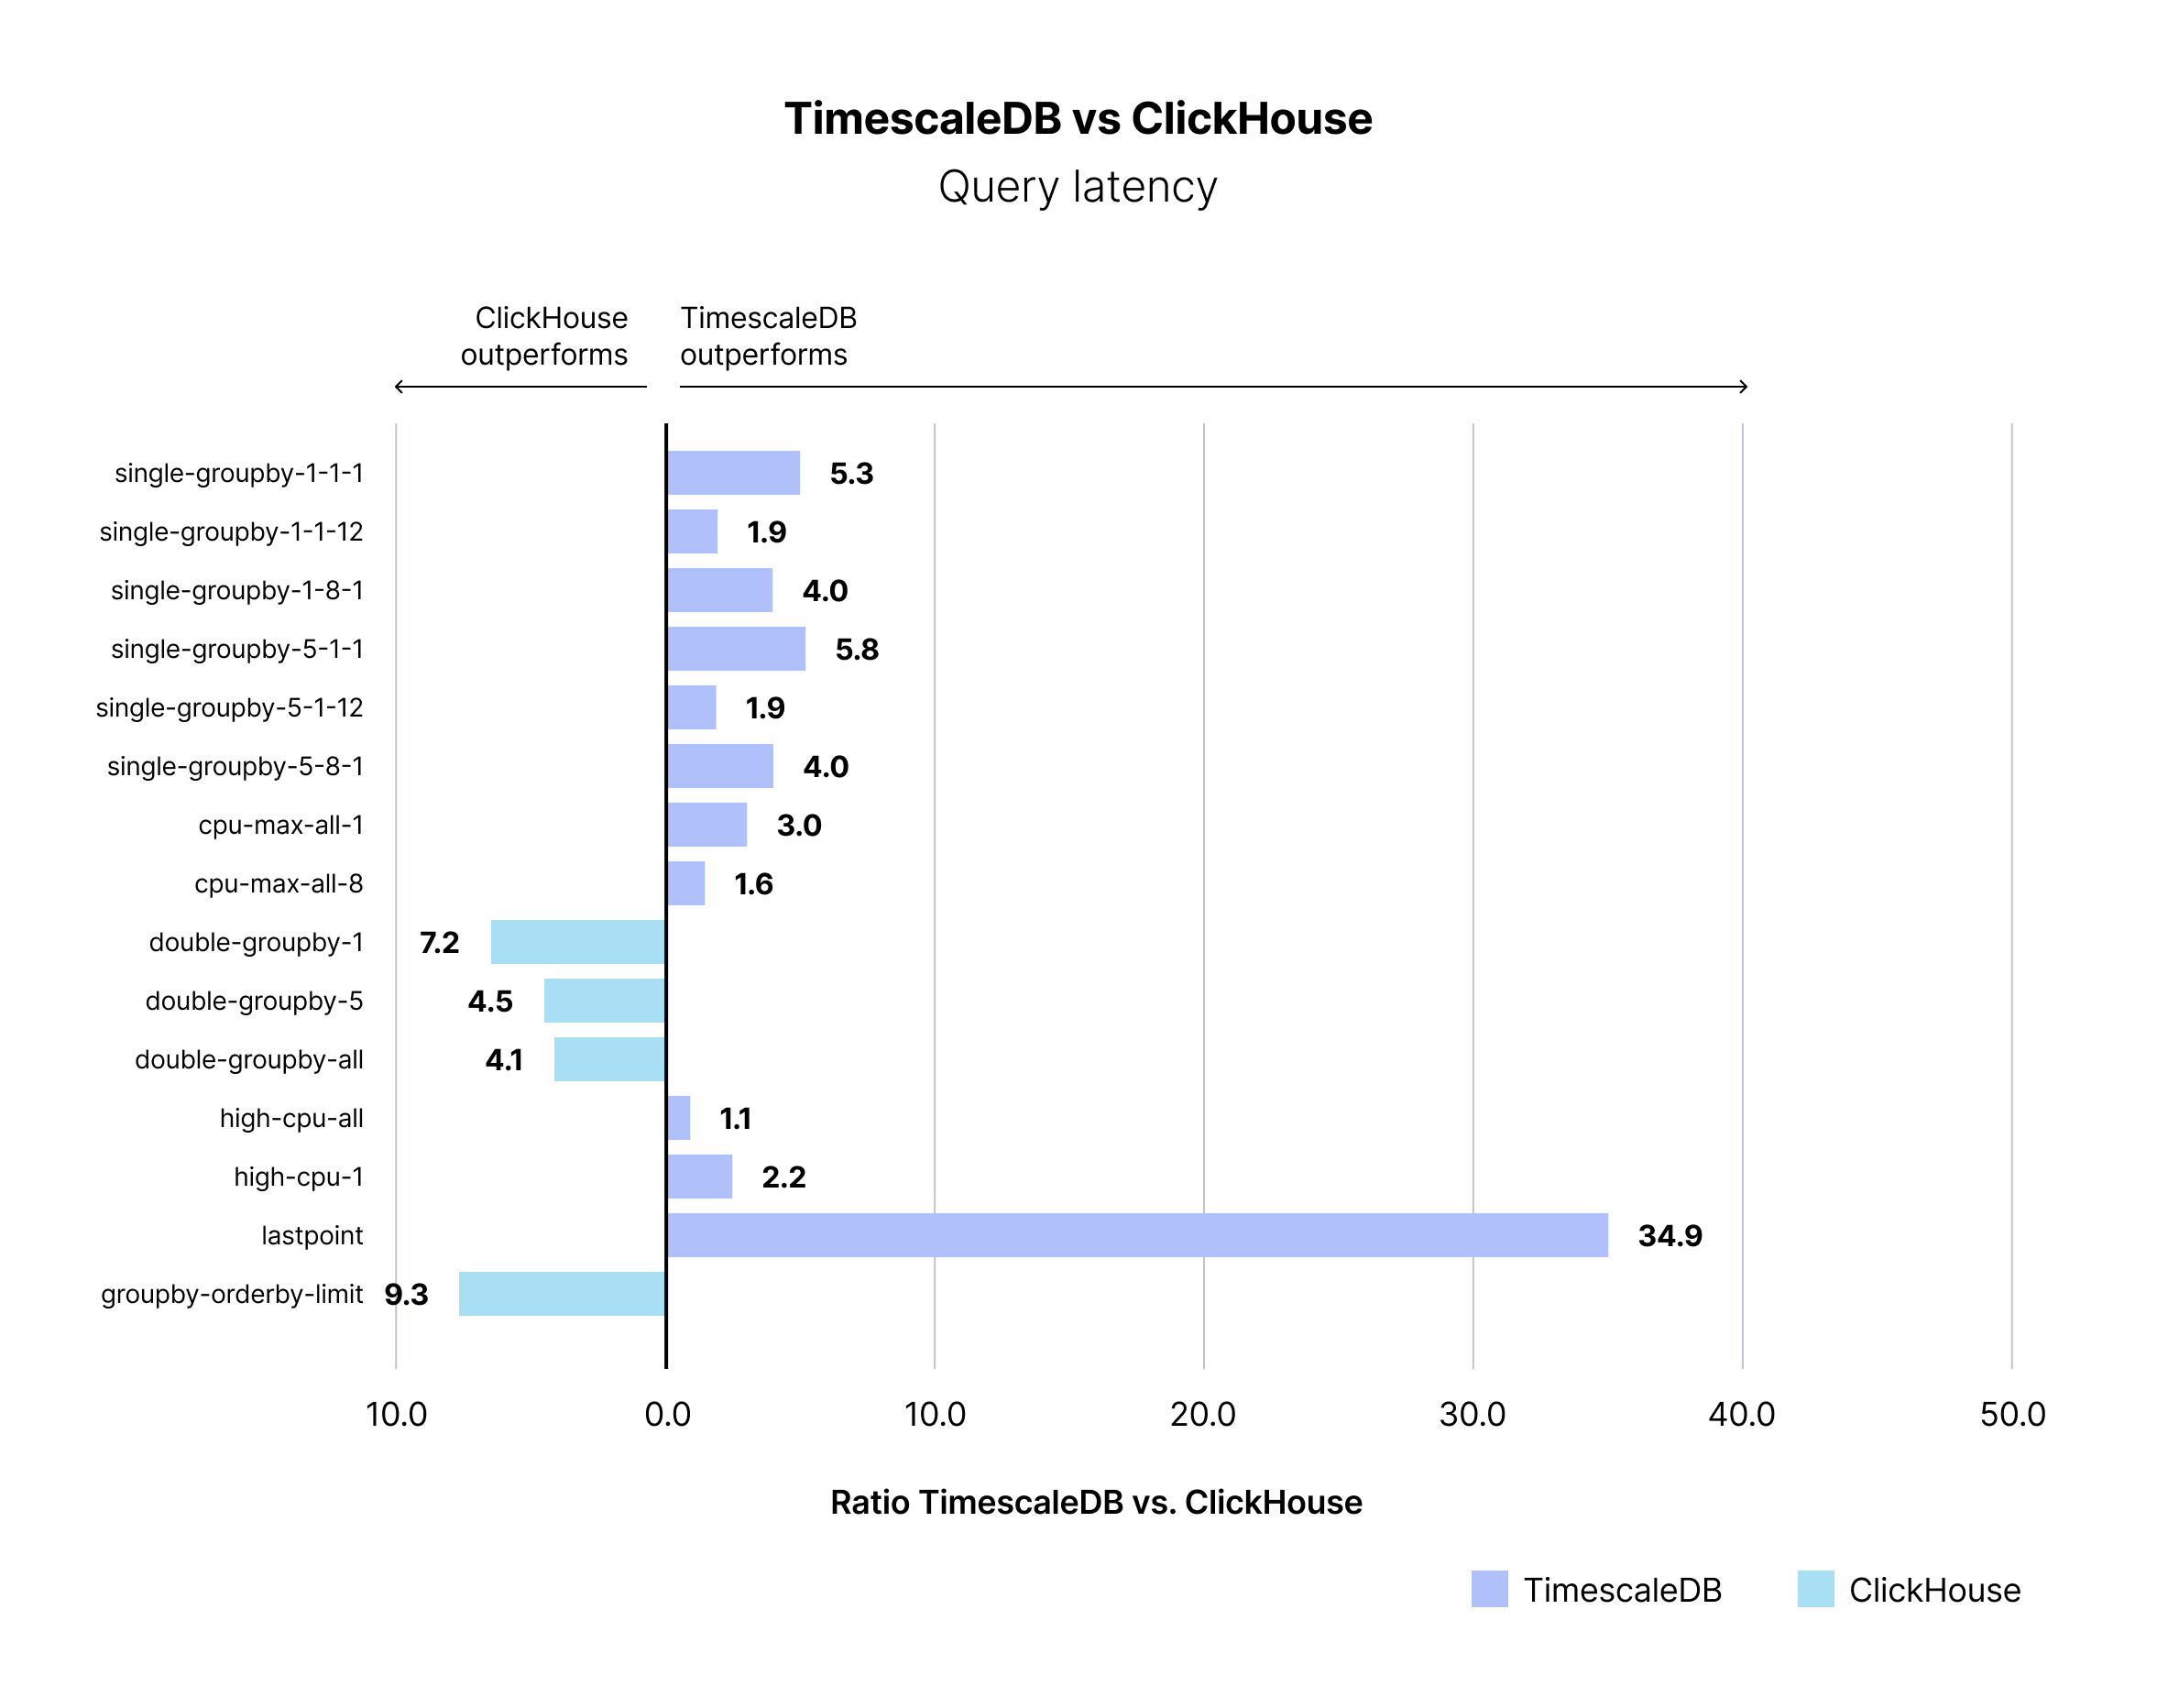
\includegraphics[width=0.85\textwidth]{imgs/03-query-latency.png}
	\captionof{figure}{\href{https://www.timescale.com/blog/what-is-clickhouse-how-does-it-compare-to-postgresql-and-timescaledb-and-how-does-it-perform-for-time-series-data/}{Performance relative alle query}}
\end{center}

\begin{center}
	\includegraphics[width=0.85\textwidth]{imgs/07-\href{https://7last.github.io/docs/pb/documentazione-interna/glossario\#clickhouse}{clickhouse\textsubscript{G}}-improvement.png}
	\captionof{figure}{\href{https://www.timescale.com/blog/what-is-clickhouse-how-does-it-compare-to-postgresql-and-timescaledb-and-how-does-it-perform-for-time-series-data/}{Performance degli insert}}
\end{center}

\begin{center}
	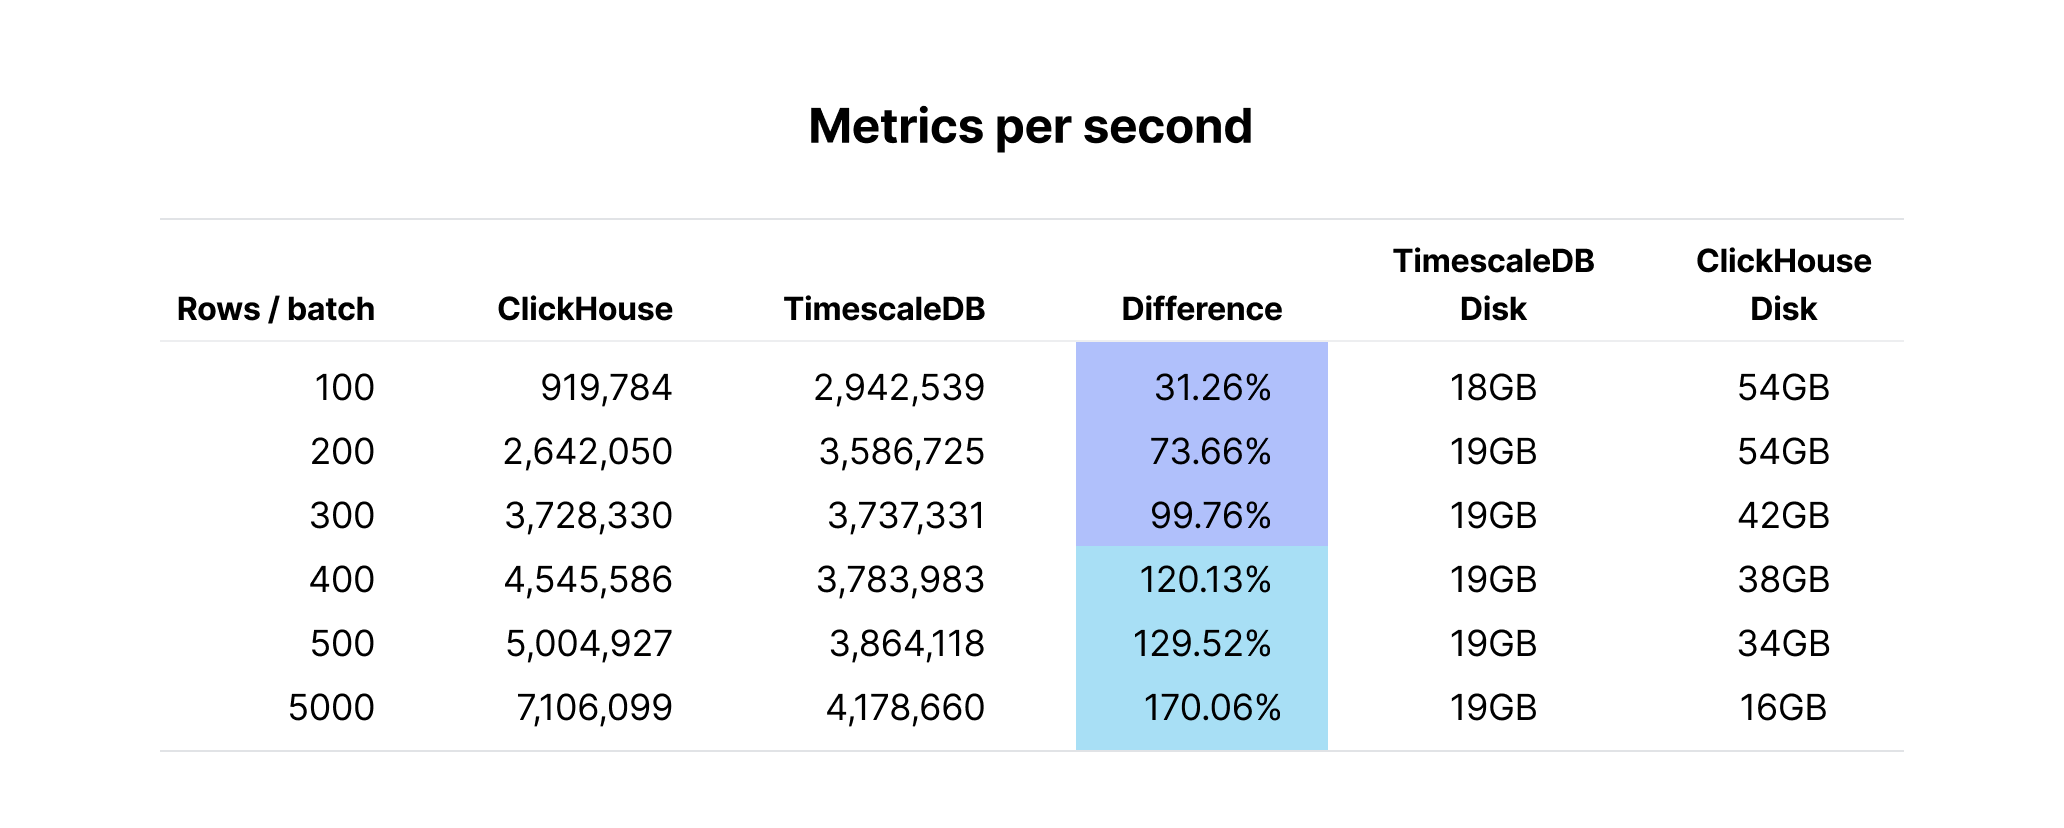
\includegraphics[width=0.85\textwidth]{imgs/08-chunk-time-interval.png}
	\captionof{figure}{\href{https://www.timescale.com/blog/what-is-clickhouse-how-does-it-compare-to-postgresql-and-timescaledb-and-how-does-it-perform-for-time-series-data/}{Performance degli insert con batch di dimensioni ridotte}}
\end{center}

\begin{center}
	\includegraphics[width=0.85\textwidth]{imgs/09-\href{https://7last.github.io/docs/pb/documentazione-interna/glossario\#clickhouse}{clickhouse\textsubscript{G}}-benchmark-read-latency-performance.png}
	\captionof{figure}{\href{https://www.timescale.com/blog/what-is-clickhouse-how-does-it-compare-to-postgresql-and-timescaledb-and-how-does-it-perform-for-time-series-data/}{Performance di query di 4000 host con 100 milioni di righe di dati}}
\end{center}

\begin{center}
	\includegraphics[width=0.85\textwidth]{imgs/10-\href{https://7last.github.io/docs/pb/documentazione-interna/glossario\#clickhouse}{clickhouse\textsubscript{G}}-benchmark-read-latency-performance.png}
	\captionof{figure}{\href{https://www.timescale.com/blog/what-is-clickhouse-how-does-it-compare-to-postgresql-and-timescaledb-and-how-does-it-perform-for-time-series-data/}{Performance di query di 10000 host con 100 milioni di righe di dati}}
\end{center}








\section{Conclusioni}
Se sono necessarie query su dataset ampi e poco mutevoli, eseguite da pochi utenti Clickhouse è la scelta adatta.
Se invece sono presenti casi d’uso tipici di un database OLTP ed è necessaria l'implementazione di time-series TimescaleDB è la soluzione.
Nel nostro caso gli ambiti di utilizzo rispecchiano pienamente quelli di ClickHouse.







\end{document}



